\section{Analyse geeigneter Prozessmodellierungssprachen}\label{analyse_sprachen}

„Von der Wahl der Modellierungssprache hängt also ab, was in einem Modell überhaupt abgebildet werden kann, und was nicht sichtbar werden kann, weil die Modellierungssprache keine Konzepte dafür anbietet.“ \cite{Fleischmann2018} Die Interviews ergaben die Notwendigkeit der Funktion, RPA-Roboter in Modellierungssprachen zu erstellen. Daher wird nachfolgend untersucht, welche Notationen sich für die Implementierung von RPA-Robotern eignen. 

\subsection{Analyse des ausführbaren RobotFramework Codes}

Betrachten wir vor der Analyse der Modellierungssprachen die Syntax der Programmiersprache RobotFramework\footnote{\url{www.robotframework.org} (Abgerufen 19. Juni 2021)}, um im Anschluss bewerten zu können, welche Programmierkonzepte von den Notationen unterstützt werden müssen. RobotFramework wurde für die Ausführung der Automatisierungen gemeinsam mit den Bibliotheken des RpaFrameworks\footnote{\url{www.rpaframework.org} (Abgerufen 19. Juni 2021)} verwendet. 

RobotFramework ist ein quellenoffenes Framework, das für die Testautomatisierung und RPA verwendet werden kann. Es bietet einen leicht lesbaren Code, mit dem auch Einsteiger Automatisierungen erstellen können. Das Framework wird aktiv weiterentwickelt und von zahlreichen Unternehmen wie beispielsweise DB~Schenker,  Capgemini, Kuka oder auch der Deutschen Post verwendet. Alle zugrunde liegenden Bibliotheken sind in Java oder Python implementiert und können daher bei Bedarf erweitert werden.\footnote{sämtliche Informationen entnommen aus: \\ \url{https://robotframework.org/\#introduction} (Abgerufen 19. Juni 2021)}

Die Bibliotheken des \mbox{RpaFrameworks} stellen die RPA-Aufrufe zur Verfügung. Die zugrunde liegende Programmierlogik wird in der Syntax der Test-Entwicklungssprache \mbox{RobotFramework} geschrieben. Daher wird sich im Verlauf der Arbeit vor allem auf diese Syntax bezogen. 

RPA-Roboter beschreiben Nutzerinteraktionen in verschiedenen Desktopanwendungen oder Browsern. Da es sich bei den Automatisierungen um ausführbare Programme handelt, besitzen diese die typischen Elemente einer jeden Programmiersprache. Somit finden sich in RobotFramework sequenzielle Anweisungen, Verzweigungen sowie terminierte Wiederholungen (implementiert als \code{FOR}- oder \code{WHILE}-Schleife). Zudem werden in RobotFramework Variablen unterstützt. Oftmals werden diese genutzt, um das Ergebnis einer RPA-Aktivität (zum Beispiel \flqq Microsoft Excel\frqq $\rightarrow$ \frqq Get Cell Value\flqq) zwischenzuspeichern und dann als Eingabeparameter einer anderen Aktivität anzugeben. Die Konzepte von Try-Catch Blöcken sind aktuell noch nicht vollumfänglich implementiert und werden daher in dieser Arbeit nicht weiter betrachtet.

Anhand eines Beispiel-Roboters, der den elektronischen Versand eines Mahnbescheides automatisiert, werden nachfolgend die theoretischen Grundlagen erläutert. Dem Roboter zugrunde liegt eine EXCEL-Tabelle, die täglich von den Mitarbeitenden der Verwaltung gefüllt wird und den Vor- und Nachnamen des Kunden, die Mail-Adresse sowie den Mahnungszähler 1 oder 2 beinhaltet. Die letzte Zahl gibt an, die wievielte Zahlungsaufforderung an den Kunden gesendet werden soll. Der Roboter öffnet jede Nacht die erstellte EXCEL-Tabelle und geht Zeile für Zeile die Einträge der Tabelle durch.\footnote{Das automatische Starten des Roboters wird aus Komplexitätsgründen nicht betrachtet.} Er ließt dafür jede Zeile einzeln ein und prüft im Anschluss den Mahnungszähler. Abhängig von der eingetragenen Zahl wird er nun eine Mail an den Kunden erstellen und mit dem entsprechenden Mahnbescheid als Anlage versehen. Sobald der Roboter am Ende der Tabelle angekommen ist, terminiert die Automatisierung und das Mail-Programm schließt sich. 

\begin{table}[h!]
    \centering
    \caption{Ausgangstabelle des Beispielprozesses}
    \begin{tabular}{|l|l|l|c|}
    \hline
    \textbf{Lastname} & \textbf{Firstname} & \textbf{Mail}      & \textbf{Counter} \\ \hline
    Stella        & Patricia         & p.stella@outlook.com       & 1                      \\ \hline
    Matthäus      & Clara            & familie-matthaeus@gmx.com  & 2                      \\ \hline
    Zenzi         & Mathis           & m.zenzi@web.de             & 1                      \\ \hline
    Reinhold      & Cornelia         & conny.reinhold@t-online.de & 1                      \\ \hline
    \end{tabular}
    \label{tab:exampleExcel}
\end{table}

Im Anhang ist der ausführbare Prozess in der Syntax des RobotFrameworks dargestellt (Abbildung \ref{fig:ScrRobotFr}). Dabei wurde an einigen Stellen auf die Verwendung von Test-Case Bezeichnungen, die im übrigen Code rosa eingefärbt sind, verzichtet. Diese Einschränkung war notwendig, da jeder Testcase einen eigenen Variablen-Scope bildet, sodass die  lokalen definierten Variablen in darauffolgenden Anschnitten nicht wiederverwendet werden können.

\subsection{Analyse der Semantik ausgewählter Notationen}

Um einen Roboter vollumfänglich in einer Modellierungssprache erstellen zu können, muss diese mindestens genau so mächtig wie die verwendete Sprache der Automatisierung (in unserem Fall RobotFramework) sein. Diese Mächtigkeit findet sich vor allem in Modellierungssprachen, die es ermöglichen, Softwareprogramme oder Geschäftsprozesse abzubilden. In diesem Abschnitt werden die sehr verständlichen und aussagekräftigen Flussdiagramme \cite{WILHELM2007} sowie die BPMN, der meist eingesetzte Standard zur Abbildung von Geschäftsprozessen \cite{Fleischmann2018}, analysiert. Zudem werden die laut einer Studie zur Verbreitung von Notationen im deutschsprachigen Europa (\autoref{fig:survey} \cite{mastersthesisLobe}) sehr bekannten Ereignisgesteuerten Prozessketten (EPK) betrachtet. Diese sind jedoch kaum spezifiziert und werden daher außerhalb des deutschsprachigen Raumes nur selten verwendet \cite{Clemente2011}.

\begin{figure}[h!]
    \centering
    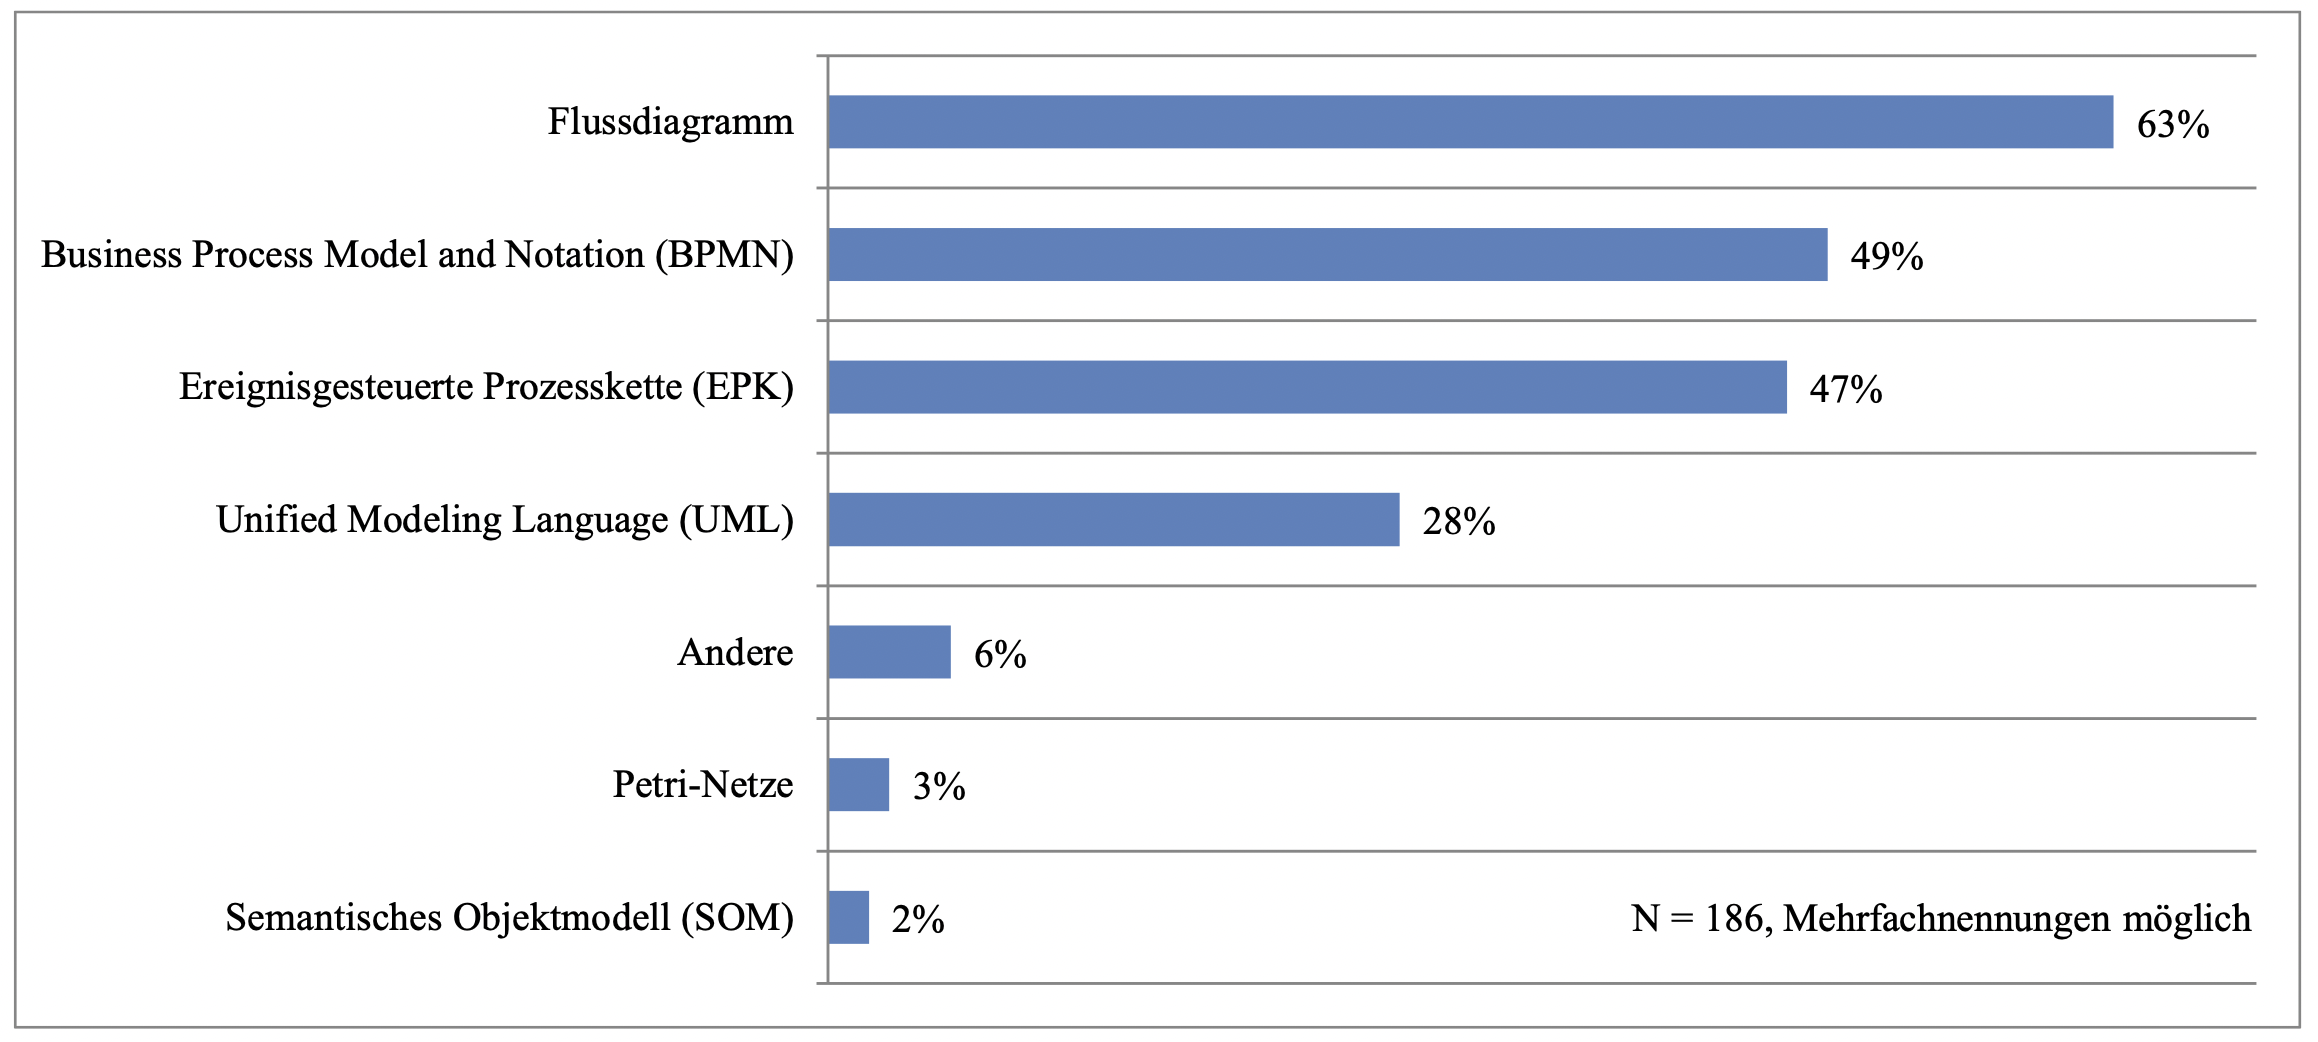
\includegraphics[width=1.03\textwidth]{images/studie_Modellierungssprachen.png}
    \caption{Verbreitung von Notationen im deutschsprachigen Europa}
    \label{fig:survey}
\end{figure}

Der finale Ausführungscode kann auch als eine Modellierungssprache angesehen werden, da er trivialerweise alle notwendigen Programmierkonzepte unterstützt. Hier soll jedoch die Betrachtung der oben genannten Sprachen genügen.

\subsubsection{Analyse des Programmablaufplans}
Der Programmablaufplan (auch oft als Flussdiagramm bezeichnet) ist in der ISO 5807 sowie DIN 66001 beschrieben. Wie in \cite{Hering1984} erläutert, dient der Programmablaufplan zur Darstellung der „Grundstruktur der Datenverarbeitung“. Es stehen so genannte „Sinnbilder“ zum Abbilden der bekannten Konzepte der Sequenz, Verzweigung sowie Wiederholung zur Verfügung. Darüber hinaus sind ebenso im Standard Kommentarfelder definiert, die an jedes Sinnbild angehangen werden können. Lediglich für Variablen existiert keine vordefinierte Syntax. Hierfür könnte jedoch das Sinnbild des Parallelogramms genutzt werden, das laut Standard Eingaben und Ausgaben definiert. 

\begin{figure}[h!]
    \centering
    % =================================================
% Set up a few colours
\colorlet{lcnorm}{black}
% -------------------------------------------------
% Set up a new layer for the debugging marks, and make sure it is on
% top
\pgfdeclarelayer{marx}
\pgfsetlayers{main,marx}
% A macro for marking coordinates (specific to the coordinate naming
% scheme used here). Swap the following 2 definitions to deactivate
% marks.
\providecommand{\cmark}[2][]{%
  \begin{pgfonlayer}{marx}
    \node [nmark] at (c#2#1) {#2};
  \end{pgfonlayer}{marx}
  } 
\providecommand{\cmark}[2][]{\relax} 
% -------------------------------------------------
% Start the picture
\begin{tikzpicture}[%
    >=triangle 60,              % Nice arrows; your taste may be different
    start chain=going below,    % General flow is top-to-bottom
    node distance=5mm and 60mm, % Global setup of box spacing
    every join/.style={norm},   % Default linetype for connecting boxes
    ]
% ------------------------------------------------- 
% A few box styles 
% <on chain> *and* <on grid> reduce the need for manual relative
% positioning of nodes
\tikzset{
  base/.style={draw, on chain, on grid, align=center, minimum height=4ex},
  proc/.style={base, rectangle, text width=8em},
  test/.style={base, diamond, aspect=2, text width=5em},
  term/.style={proc, rounded corners},
  circ/.style={base, circle},
  % coord node style is used for placing corners of connecting lines
  coord/.style={coordinate, on chain, on grid, node distance=6mm and 25mm},
  % nmark node style is used for coordinate debugging marks
  nmark/.style={draw, cyan, circle, font={\sffamily\bfseries}},
  % -------------------------------------------------
  % Connector line styles for different parts of the diagram
  norm/.style={->, draw, lcnorm},
  free/.style={->, draw, lcfree},
  cong/.style={->, draw, lccong},
  it/.style={font={\small\itshape}}
}
% -------------------------------------------------
% Start by placing the nodes
% Use join to connect a node to the previous one 
\node [term]       (te1){Robot Started};
\node [proc, join] (p1) {Open Excel};
\node [proc, join]      {Open Outlook};
\node [proc, join]      {Get Data from Excel};
\node [circ, join] (c1) {};
\node [proc, join] (p2) {Log \$\{row\}};
\node [proc, join] (p3) {Get Lastname};
\node [proc, join] (p4) {Get Firstname};
\node [proc, join] (p5) {Get Mail};
\node [proc, join] (p6) {Get Counter};
\node [test, below right = 5em and 19em of te1] (t1) {};
\node [proc, below left  = 3em and 8em of t1] (p7) {Send Reminder1};
\node [proc, below right = 3em and 8em of t1] (p8) {Send Reminder2};
\node [circ, below= 5.5em of t1] (c2) {};
\node [test, join] (t2) {};
\node [proc, join] (p9) {Close Outlook};
\node [proc, join] (p10){Close Excel};
\node [term, join]      {Robot \\ Terminated};

% -------------------------------------------------
\path (t1.west) to node [near start, xshift=-3.5em, yshift=1.2em] {IF \$\{counter\} == 1} (p7); 
  \draw [->,lcnorm] (t1.west) -| (p7.north);
\path (t1.east) to node [near start, xshift=3.5em, yshift=1.2em] {IF \$\{counter\} == 2} (p8); 
  \draw [->,lcnorm] (t1.east) -| (p8.north);
\path (p7.south) to node [near start, xshift=2em, yshift=1em] {} (p7); 
  \draw [->,lcnorm] (p7.south) |- (c2);
\path (p8.south) to node [near start, xshift=2em, yshift=1em] {} (p8); 
  \draw [->,lcnorm] (p8.south) |- (c2);

\draw [->] (p6.south) -- ++(0mm,-4mm)  -- ++(23mm,0) -- ++(0mm,113mm)
  -| (t1.north);
\draw [->] (t2.east) -- ++(35mm,0mm)  -- ++(0,55mm) -- ++(-101mm,0mm)
   |- (c1.east);
\end{tikzpicture}
    %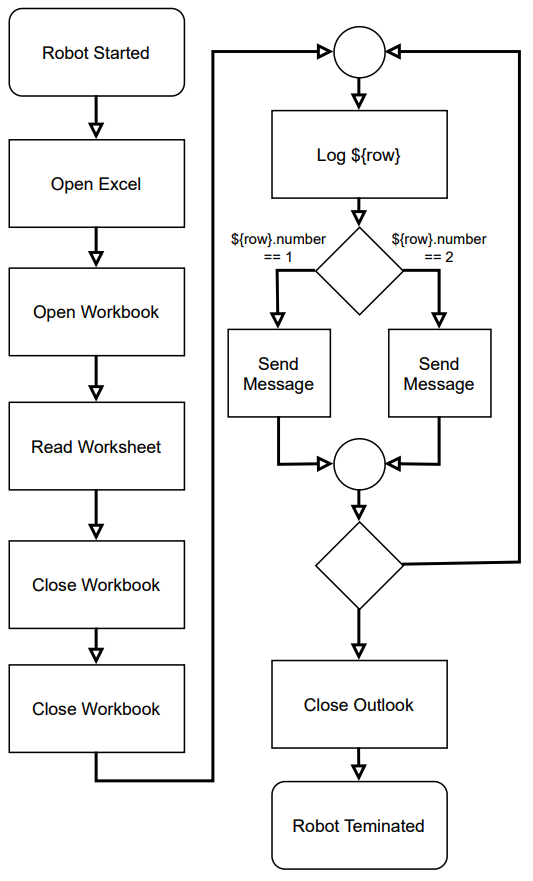
\includegraphics[width=0.5\textwidth]{Bachelorarbeit/images/ScreenshotFlowchart.png}
    \caption{Beispielprozess in Flowchart-Syntax}
    \label{fig:ScrFlow}
\end{figure}

Wie in der Abbildung \ref{fig:ScrFlow} zu sehen, eignen sich Flussdiagramme (engl. Flowchart) sehr gut für die Darstellung eines Softwareroboters. Der Arbeit ist eine Auflistung der elementaren logischen Ablaufstrukturen aus dem Werk von E. Hering \cite{Hering1984} beigefügt (Abbildung \ref{fig:UebersichtFlowchart}).

\subsubsection{Analyse der BPMN}
Wie in Abbildung \ref{fig:ScrBPMN} gezeigt, können sequenzielle Anweisungen in BPMN als Folge von Aktivitäten dargestellt werden. Verzweigungen lassen sich als XOR-Split mit entsprechenden Fallbedingungen abbilden. Ebenso können mit einem XOR-Split  Wiederholungen implementiert werden. Sofern Variablen auch in der visuellen Repräsentation sichtbar werden sollen, lassen sich diese durch Datenobjekte darstellen. 

\begin{figure}[h!]
    \centering
    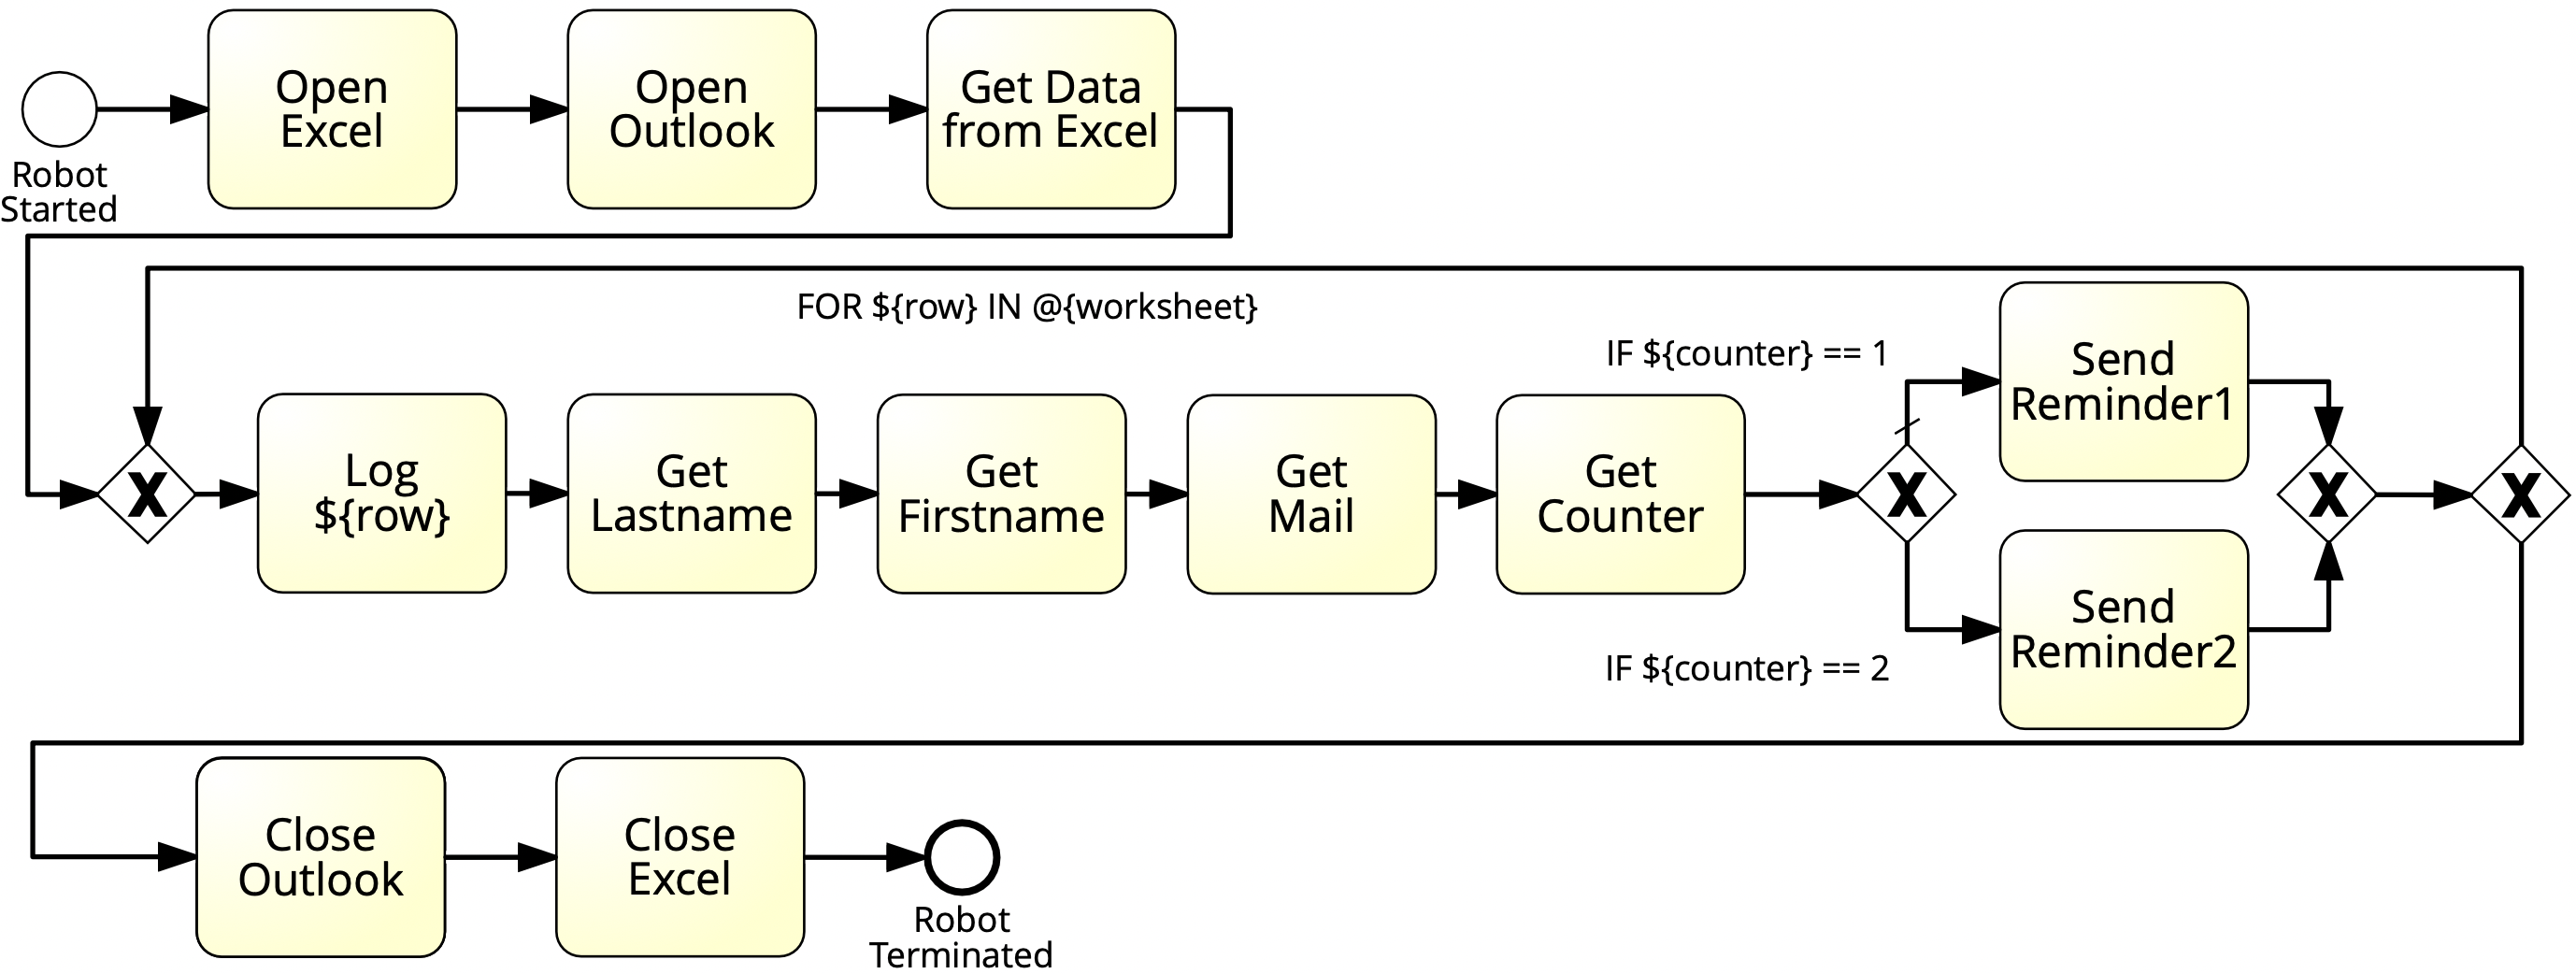
\includegraphics[width=1.0\textwidth]{Bachelorarbeit/images/ScreenshotBPMN4.png}
    \caption{Beispielprozess in BPMN-Syntax}
    \label{fig:ScrBPMN}
\end{figure}

Ursprünglich ist die Prozessmodellierungssprache BPMN nicht dafür konzipiert worden, Softwareabläufe darzustellen. Wie soeben gezeigt, eignet sich die Notation neben der Prozessmodellierung auch für die Implementierung von RPA-Robotern. Zudem bietet sie bereits im Standard die Möglichkeit alle Aktivitäten zu dokumentieren. Dieses Feature wurde von den RPA-Entwicklern ausdrücklich gewünscht und gilt als ein zentraler Vorteil der BPMN und des Programmablaufplans gegenüber anderen Prozessmodellierungssprachen.

\subsubsection{Analyse der EPK}

Die Ereignisgesteuerte Prozesskette wurde an der Universität des Saarlandes zusammen mit der SAP AG zur Dokumentation von Geschäftsprozessen entwickelt \cite{epkSyntax}.
Die EPK besitzt als Kernelemente das Ereignis, das einen Zustand im Prozess abbildet sowie die Funktion, die eine Aktion oder Aufgabe beschreibt. Jeder Prozess startet und endet mit einem Ereignis. Zwischen beiden Ereignissen können sequenzielle Anweisungen durch aneinandergereihte Funktionsaufrufe dargestellt werden. Durch Einsatz des XOR-Konnektors lassen sich analog zur BPMN (\mbox{Abbildung \ref{fig:ScrEPK}}) Verzweigungen sowie Schleifen darstellen.  Hierbei ist zu beachten, dass nach jeder XOR-Verzweigung zwingend ein Ereignis folgen muss, um den vorliegenden Zustand zu beschreiben. Diese Ereignis-Elemente dienen in unserem Fall zur Angabe der Fallbedingungen einer Verzweigung oder zur Darstellung der Schleifenabbruchbedingung.

\begin{figure}[h!]
    \centering
    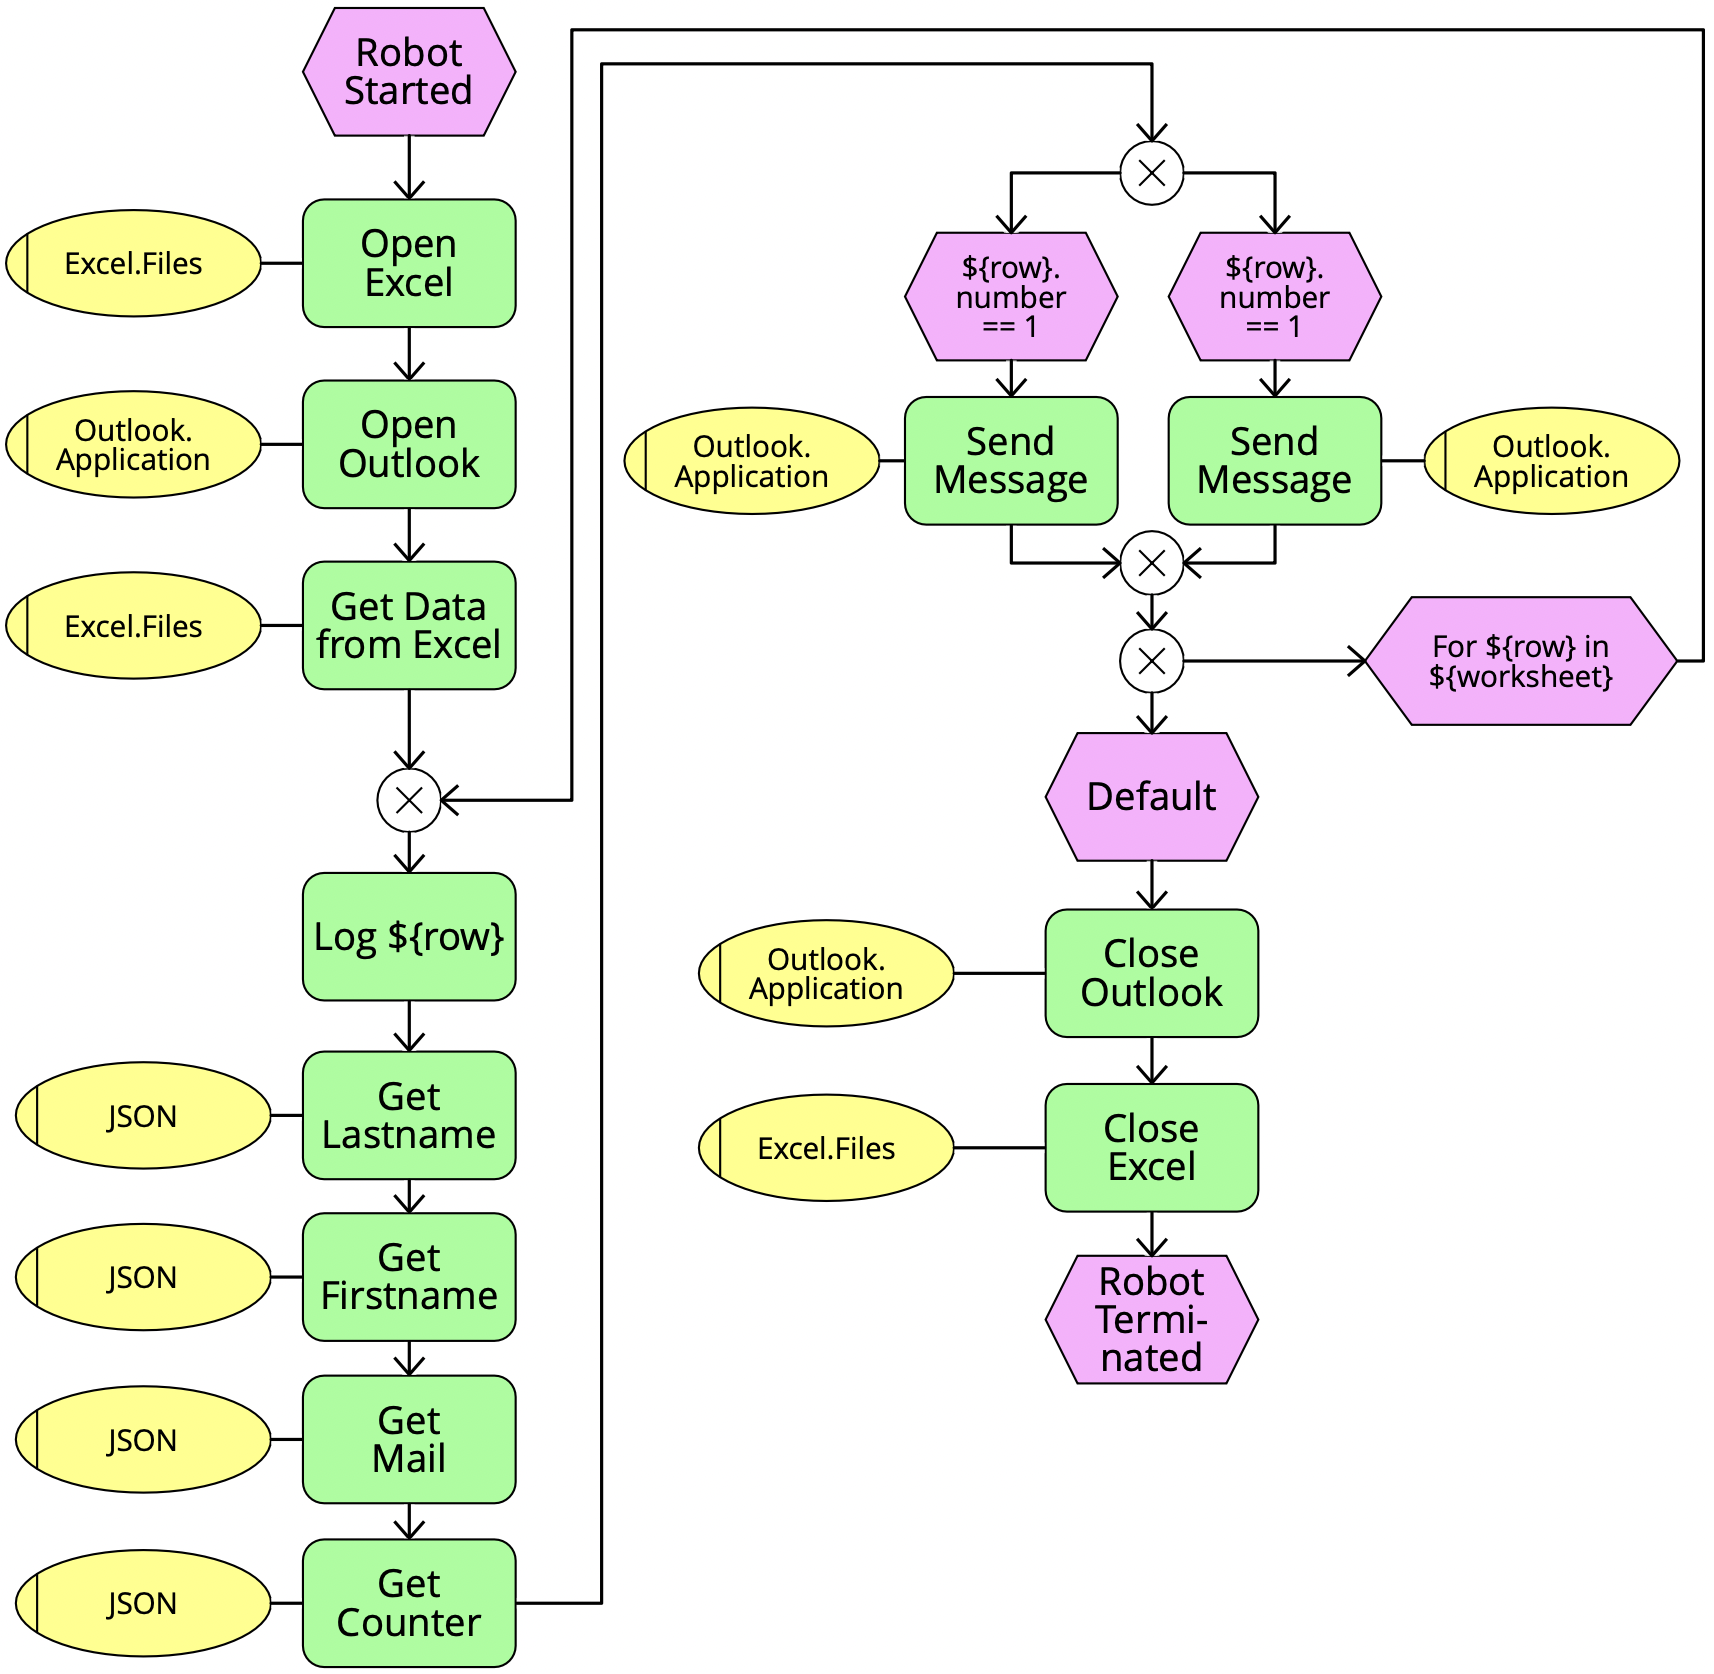
\includegraphics[width=0.75\textwidth]{Bachelorarbeit/images/ScreenshotEPK3.png}
    \caption{Beispielprozess in EPK-Syntax}
    \label{fig:ScrEPK}
\end{figure}

Wie beschrieben, lassen sich auch mit EPKs RPA-Roboter darstellen. Ähnlich zur BPMN können dem Diagramm Datenobjekte hinzugefügt und dadurch Variablen repräsentiert werden. Darüber hinaus lässt das „Organisationseinheit“-Element für die Darstellung der zum Ausführen der RPA-Aufgabe genutzten Anwendung (z.B. \code{Excel.Application}) verwenden. Dieses zusätzliche Element kann in der jedoch auch Visualisierung kann jedoch entfernt werden, da zu jeder Funktion die RPA-Anwendung gesondert im Seitenmenü spezifiziert werden muss.